% Preâmbulo: Configuração inicial do documento com pacotes compatíveis
\documentclass[12pt, a4paper]{article}
\usepackage[utf8]{inputenc}
\usepackage[T1]{fontenc}
\usepackage[portuguese]{babel}
\usepackage{geometry}
\usepackage{setspace}
\usepackage{indentfirst}
\usepackage{titlesec}
\usepackage{tocloft}
\usepackage{amsmath}
\usepackage{svg}
\usepackage{float}
\usepackage{graphicx}
\usepackage{listings}
\usepackage{xcolor}
\usepackage{hyperref}
\usepackage{enumitem}

% Configuração de margens conforme ABNT NBR 14724:2011
\geometry{left=3cm, right=2cm, top=3cm, bottom=2cm}

% Configuração de espaçamento e fonte
\onehalfspacing
\renewcommand{\familydefault}{\rmdefault}

% Configuração de títulos conforme ABNT
\titleformat{\section}{\normalfont\large\bfseries}{\thesection}{1em}{}
\titleformat{\subsection}{\normalfont\normalsize\bfseries}{\thesubsection}{1em}{}
\titleformat{\subsubsection}{\normalfont\normalsize\bfseries}{\thesubsubsection}{1em}{}

% Configuração do sumário
\renewcommand{\cftsecleader}{\cftdotfill{\cftdotsep}}
\renewcommand{\cftsecdotsep}{\cftdot}
\setlength{\cftbeforesecskip}{0.5em}
\setlength{\cftbeforesubsecskip}{0.2em}

% Configuração de hiperlinks
\hypersetup{
    colorlinks=true,
    linkcolor=black,
    urlcolor=blue,
    citecolor=black
}

% Configuração para listagens de código
\lstset{
    basicstyle=\ttfamily\small,
    breaklines=true,
    frame=single,
    numbers=left,
    numberstyle=\tiny,
    keywordstyle=\color{blue},
    stringstyle=\color{red},
    commentstyle=\color{gray},
    showstringspaces=false
}

\begin{document}

% --- Capa ---
\begin{titlepage}
    \centering
    \vspace*{1cm}
    {\large\bfseries CENTRO UNIVERSITÁRIO\\ CATÓLICA DE SANTA CATARINA\\
    POLO JOINVILLE\\
    CURSO DE ENGENHARIA DE SOFTWARE}\par
    \vspace{2cm}
    {\Large\bfseries FAZENDAPRO - GERENCIADOR DE PECUÁRIA COM FOCO EM LEITE}\par
    \vspace{2cm}
    {\normalsize\bfseries Gustavo Henrique Dias}\par
    \vspace{1cm}
    \vspace{3cm}
    {\normalsize JOINVILLE\\
    18 DE JUNHO DE 2025}\par
\end{titlepage}

% --- Sumário ---
\tableofcontents
\newpage

% --- Resumo ---
\section*{Resumo}
\addcontentsline{toc}{section}{Resumo}
\begin{spacing}{1.5}
O projeto FazendaPro é uma plataforma desenvolvida como projeto para otimizar a gestão de rebanhos bovinos, com ênfase na pecuária leiteira. O sistema propõe uma interface técnica e funcional para o gerenciamento integrado de animais, pastagens e produção de leite, fornecendo ferramentas para monitoramento detalhado e análise de dados. Suas principais funcionalidades incluem o registro do histórico genético, sanitário e produtivo do gado, com foco especial no acompanhamento de vacas em lactação para otimizar a produção leiteira e identificar anomalias. O projeto visa atender às necessidades de pequenos e médios produtores, promovendo eficiência operacional e rastreabilidade no setor agropecuário.
\end{spacing}
\vspace{0.5cm}
\textbf{Palavras-chave:} Gestão pecuária, Pecuária leiteira, Rastreabilidade, Produção de leite, Tecnologia agropecuária.
\newpage

% --- Introdução ---
\section{Introdução}

\subsection{Contexto}
\begin{spacing}{1.5}
O projeto FazendaPro é desenvolvido no âmbito da pecuária brasileira, com foco na gestão de rebanhos bovinos e ênfase na produção leiteira, um setor de relevância econômica que responde por cerca de 20\% do PIB agropecuário nacional \cite{agro20}. Apesar de sua importância, pequenos e médios produtores enfrentam desafios significativos, como a dependência de métodos manuais ou planilhas para gestão, resultando em ineficiências, falta de rastreabilidade do histórico genético e sanitário dos animais, dificuldades na previsão de produtividade leiteira e custos operacionais elevados. Segundo a Embrapa, Empresa Brasileira de Pesquisa Agropecuária,  aproximadamente 80\% dos produtores leiteiros brasileiros utilizam práticas tradicionais de baixa tecnologia, o que limita a competitividade e a eficiência \cite{anuario2023}. No norte de Minas Gerais, por exemplo, produtores relatam dificuldades em valorizar seus animais no mercado devido à ausência de registros detalhados, conforme noticiado pelo portal G1 \cite{g12022}.
\end{spacing}

\subsection{Justificativa}
\begin{spacing}{1.5}
O desenvolvimento do FazendaPro justifica-se pela necessidade de modernizar a gestão pecuária, com foco na pecuária leiteira, para pequenos e médios produtores que enfrentam barreiras no acesso à tecnologias avançadas. A pecuária leiteira é uma atividade econômica essencial, empregando cerca de 4 milhões de pessoas no Brasil \cite{4milhao}. Um produtor do norte de Minas Gerais relatou perdas na comercialização de animais devido à ausência de registros detalhados sobre genética e saúde, conforme destacado em reportagem do G1 \cite{g12022}. Além disso, sistemas comerciais existentes frequentemente apresentam custos elevados e interfaces inadequadas às necessidades rurais, conforme apontado análise pelo blog Agrolink \cite{agropec2024}. O FazendaPro, como projeto acadêmico, propõe uma solução técnica, acessível e escalável, com ênfase na rastreabilidade de rebanhos e no monitoramento da produção leiteira, contribuindo para a eficiência operacional, a valorização do gado e a sustentabilidade do setor.
\end{spacing}

\subsection{Objetivos}
\begin{spacing}{1.5}
\subsubsection{Objetivo Principal}
Desenvolver uma plataforma digital para a gestão integrada de rebanhos bovinos, com foco na pecuária leiteira, que permita o registro detalhado do histórico genético, sanitário e produtivo dos animais, promovendo a rastreabilidade e a eficiência na produção de leite.

\subsubsection{Objetivos Secundários}
\begin{enumerate}[label=\alph*)]
    \item Desenvolver um sistema acessível e de baixo custo para pequenos e médios produtores rurais, não passando de 10 mil reais;
    \item Implementar funcionalidades para monitoramento em tempo real da produção de leite e da saúde animal;
    \item Automatizar processos operacionais, como notificações de prenhez e gerenciamento de lotes, reduzindo a dependência de tarefas manuais;
    \item Fornecer dashboards analíticos com dados de desempenho para apoiar a tomada de decisão;
    \item Habilitar a exportação de históricos em PDF para facilitar a comercialização de animais;
    \item Desenvolver uma interface responsiva e funcional, otimizada para dispositivos móveis.
\end{enumerate}

% --- Descrição do Projeto ---
\section{Descrição do Projeto}

\subsubsection{Problemas a Resolver}
\begin{enumerate}[label=\alph*)]
    \item \textbf{Falta de rastreabilidade}: ausência de registros estruturados sobre o histórico dos animais (nascimento, vacinação, produção etc.).
    \item \textbf{Baixa eficiência na gestão}: controle manual ou informal dificulta decisões baseadas em dados.
\end{enumerate}

\subsection{Limitações}
\begin{spacing}{1.5}
O projeto FazendaPro apresenta as seguintes limitações, identificadas com base no escopo e nos requisitos definidos:

\begin{enumerate}[label=\alph*)]
    \item \textbf{Dependência de Conectividade à Internet}: A aplicação web requer conexão estável, o que pode ser um desafio em áreas rurais com acesso limitado à internet, impactando funcionalidades como monitoramento em tempo real e notificações via WhatsApp.
    \item \textbf{Foco Primário na Pecuária Leiteira}: Embora o sistema contemple a gestão geral de rebanhos bovinos, seu foco principal é a pecuária leiteira, limitando a aplicabilidade a outros tipos de pecuária ou atividades agrícolas.
    \item \textbf{Dependência de Serviços de Terceiros}: A utilização de Google Cloud, Cloud SQL e WhatsApp introduz riscos relacionados a custos e disponibilidade.
\end{enumerate}
\end{spacing}

% --- Especificação Técnica ---
\section{Especificação Técnica}

\subsection{Requisitos Funcionais (RF)}
\begin{spacing}{1.5}
\begin{enumerate}[label=RF0\arabic{*}.]
    \item \textbf{Acessar o Sistema}
    \begin{enumerate}[label=RF01.0\arabic{*}]
        \item O sistema deve permitir que o usuário faça o login na plataforma com suas credenciais, que são fornecidas pelos desenvolvedores do software.
        \item O sistema deve validar as credenciais do usuário e conceder acesso apenas para os usuários que geraram o token (\textit{JSON Web Token}).
    \end{enumerate}
    \item \textbf{Adicionar um Animal}
    \begin{enumerate}[label=RF02.0\arabic{*}]
        \item O sistema deve permitir que o usuário cadastre um novo animal no sistema.
        \item O sistema deve permitir incluir dados do animal como, no mínimo: identificação (nome e número do brinco), data de nascimento, genitora, filho (caso exista), raça, sexo e informações de saúde (vacinas).
    \end{enumerate}
    \item \textbf{Gerenciar o Animal}
    \begin{enumerate}[label=RF03.0\arabic{*}]
        \item O sistema deve permitir que o usuário edite as informações de um animal já cadastrado.
        \item O sistema deve oferecer a opção de exportar o histórico do animal em formato PDF.
    \end{enumerate}
    \item \textbf{Inserir Informações do Animal}
    \begin{enumerate}[label=RF04.0\arabic{*}]
        \item O sistema deve permitir que o usuário insira informações adicionais sobre o animal, como registros de vacinas, alimentação, tratamentos ou eventos, como nascimento de filhotes.
    \end{enumerate}
    \item \textbf{Registrar Peso do Animal por Mês/Semana}
    \begin{enumerate}[label=RF05.0\arabic{*}]
        \item O sistema deve permitir que o usuário registre o peso do animal em intervalos regulares (mensal ou semanal).
        \item O sistema deve armazenar esses registros para acompanhamento do desenvolvimento do animal.
        \item O sistema deve permitir a edição ou exclusão desses registros.
    \end{enumerate}
    \item \textbf{Mudar de Lote}
    \begin{enumerate}[label=RF06.0\arabic{*}]
        \item O sistema deve mudar automaticamente o lote ao qual um animal pertence com base em sua produção de leite ou outros critérios configuráveis.
    \end{enumerate}
    \item \textbf{Definir Data de Prenhez}
    \begin{enumerate}[label=RF07.0\arabic{*}]
        \item O sistema deve permitir que o usuário registre a data de prenhez de uma vaca.
        \item O sistema deve notificar o usuário (via WhatsApp) quando a data de prenhez estiver próxima do parto, 20 dias antes.
    \end{enumerate}
    \item \textbf{Vender o Animal}
    \begin{enumerate}[label=RF8.0\arabic{*}]
        \item O sistema deve permitir que o usuário registre a venda de um animal.
        \item O sistema deve atualizar o status do animal para ``vendido'' e registrar a data da venda.
        \item O sistema deve oferecer a opção de exportar o histórico do animal em PDF no momento da venda.
        \item O sistema deve permitir verificar o histórico de todas as vendas dentro do módulo de vendas.
    \end{enumerate}
    \item \textbf{Cadastrar Vacinas}
    \begin{enumerate}[label=RF9.0\arabic{*}]
        \item O sistema deve permitir que o usuário cadastre vacinas para posterior vinculação aos animais.
        \item O sistema deve permitir a pesquisa de vacinas por datas.
    \end{enumerate}
    \item \textbf{Sair da Plataforma}
    \begin{enumerate}[label=RF10.0\arabic{*}]
        \item O sistema deve permitir que o usuário faça o logout da plataforma.
    \end{enumerate}
\end{enumerate}
\end{spacing}

\subsection{Requisitos Não Funcionais (RNF)}
\begin{spacing}{1.5}
\begin{enumerate}[label=RNF0\arabic{*}.]
    \item \textbf{Estilização}
    \begin{enumerate}[label=RNF01.0\arabic{*}]
        \item A estilização da aplicação deve seguir os padrões de estilo dos componentes da biblioteca Ant Design.
        \item Para facilitar a estilização, deve ser usado Tailwind ou outra biblioteca de CSS.
        \item Componentes padrões devem ser criados para seguir um padrão geral.
        \item As cores da aplicação devem apresentar-se de forma funcional e acessível.
    \end{enumerate}
    \item \textbf{Ferramentas}
    \begin{enumerate}[label=RNF02.0\arabic{*}]
        \item Para o frontend, deve-se utilizar React com bibliotecas para facilitar o fetch de informações.
        \item Para o backend, será usado NestJS para autenticação e notificações, enquanto Go será utilizado para as demais funcionalidades.
    \end{enumerate}
    \item \textbf{Idiomas}
    \begin{enumerate}[label=RNF03.0\arabic{*}]
        \item Todo o desenvolvimento deve respeitar variáveis de idioma.
        \item O idioma principal será PT-BR, com possibilidade de implementação futura de EN-US e ES-ES.
    \end{enumerate}
    \item \textbf{Separar Módulo}
    \begin{enumerate}[label=RF04.0\arabic{*}]
        \item O sistema deve organizar as informações em módulos acessíveis via menu lateral (Dashboard, Animais, Fornecedores, Vendas, Estoque).
    \end{enumerate}
    \item \textbf{Analisar Dashboards}
    \begin{enumerate}[label=RF05.0\arabic{*}]
        \item O sistema deve fornecer dashboards com informações analíticas sobre os animais, como produção de leite, saúde geral e tendências de desempenho.
    \end{enumerate}
    \item \textbf{Desempenho}
    \begin{enumerate}[label=RNF06.0\arabic{*}]
        \item O sistema deve ter tempo de resposta inferior a 2 segundos para operações básicas (CRUD).
        \item O sistema deve carregar a página inicial em menos de 3 segundos.
        \item O sistema deve processar relatórios complexos em menos de 10 segundos.
    \end{enumerate}
    \item \textbf{Otimizações Móveis}
    \begin{enumerate}[label=RNF07.0\arabic{*}]
        \item O sistema deve implementar lazy loading para imagens e componentes.
        \item O sistema deve comprimir assets CSS/JS em produção.
        \item O sistema deve implementar Progressive Web App (PWA) para melhor experiência móvel.
    \end{enumerate}
    \item \textbf{Conformidade e Privacidade}
    \begin{enumerate}[label=RNF08.0\arabic{*}]
        \item O sistema deve estar em conformidade com a LGPD para tratamento de dados.
        \item O sistema deve implementar anonimização de dados sensíveis em relatórios.
    \end{enumerate}
    \item \textbf{Conformidade com LGPD}
    \begin{enumerate}[label=RNF09.0\arabic{*}]
        \item O sistema deve implementar mecanismos de consentimento explícito para coleta e uso de dados sensíveis dos animais.
        \item O sistema deve permitir que o usuário visualize, edite e exclua dados pessoais conforme direitos da LGPD.
        \item O sistema deve permitir a exportação de dados em formato legível conforme direito de portabilidade.
    \end{enumerate}
\end{enumerate}
\end{spacing}

\subsection{Diagrama de Casos de Uso}
\begin{spacing}{1.5}
O diagrama de casos de uso está apresentado na Figuras 1, 2, 3, 4 e 5. Nela busca-se explicar um pouca da história do usuário através das principais funcionalidade e ideais do sistema. Nesse exemplo, o usuário acessará o sistema e poderá gerenciar ou cadastrar o animal, independente da decisão ele terá que fornecer as informações do animal, como idade, raça, etc.
\begin{figure}[H]
    \centering
    \includegraphics[width=0.8\textwidth]{diagrams/cases-of-use-8-new.drawio.png}
    \caption{Diagrama de Casos de Uso - Gerenciador do Animal}
    \label{fig:cases-of-use}
\end{figure}

\begin{figure}[H]
    \centering
    \includegraphics[width=0.8\textwidth]{diagrams/cases-of-use-6-new.drawio.png}
    \caption{Diagrama de Casos de Uso - Prenhez}
    \label{fig:cases-of-use}
\end{figure}
\end{spacing}
Poderá também fazer o registro do peso do animal já existente, e caso respeite a regra específica, o animal é trocado de lote por um worker.

\begin{figure}[H]
    \centering
    \includegraphics[width=1\textwidth]{diagrams/cases-of-use-7-new.drawio.png}
    \caption{Diagrama de Casos de Uso - Movimentação}
    \label{fig:cases-of-use}
\end{figure}

 O usuário poderá visualizar o histórico do animal e vendê-lo.

\begin{figure}[H]
    \centering
    \includegraphics[width=0.8\textwidth]{diagrams/cases-of-use-4.drawio.png}
    \caption{Diagrama de Casos de Uso - Venda}
    \label{fig:cases-of-use}
\end{figure}
\end{spacing}

\begin{figure}[H]
    \centering
    \includegraphics[width=0.8\textwidth]{diagrams/cases-of-use-5-new.drawio.png}
    \caption{Diagrama de Casos de Uso - Relatórios}
    \label{fig:cases-of-use}
\end{figure}
\end{spacing}

\subsection{Diagrama de Classes}
\begin{spacing}{1.5}
O diagrama de classes está apresentado na Figura \ref{fig:classes-diagram}. Nele pode-se encontrar a fluxo das classes que será representado a nível de código. Ajuda o desenvolvedor a criar e visualizar as classes com maior facilidade.
\begin{figure}[H]
    \centering
    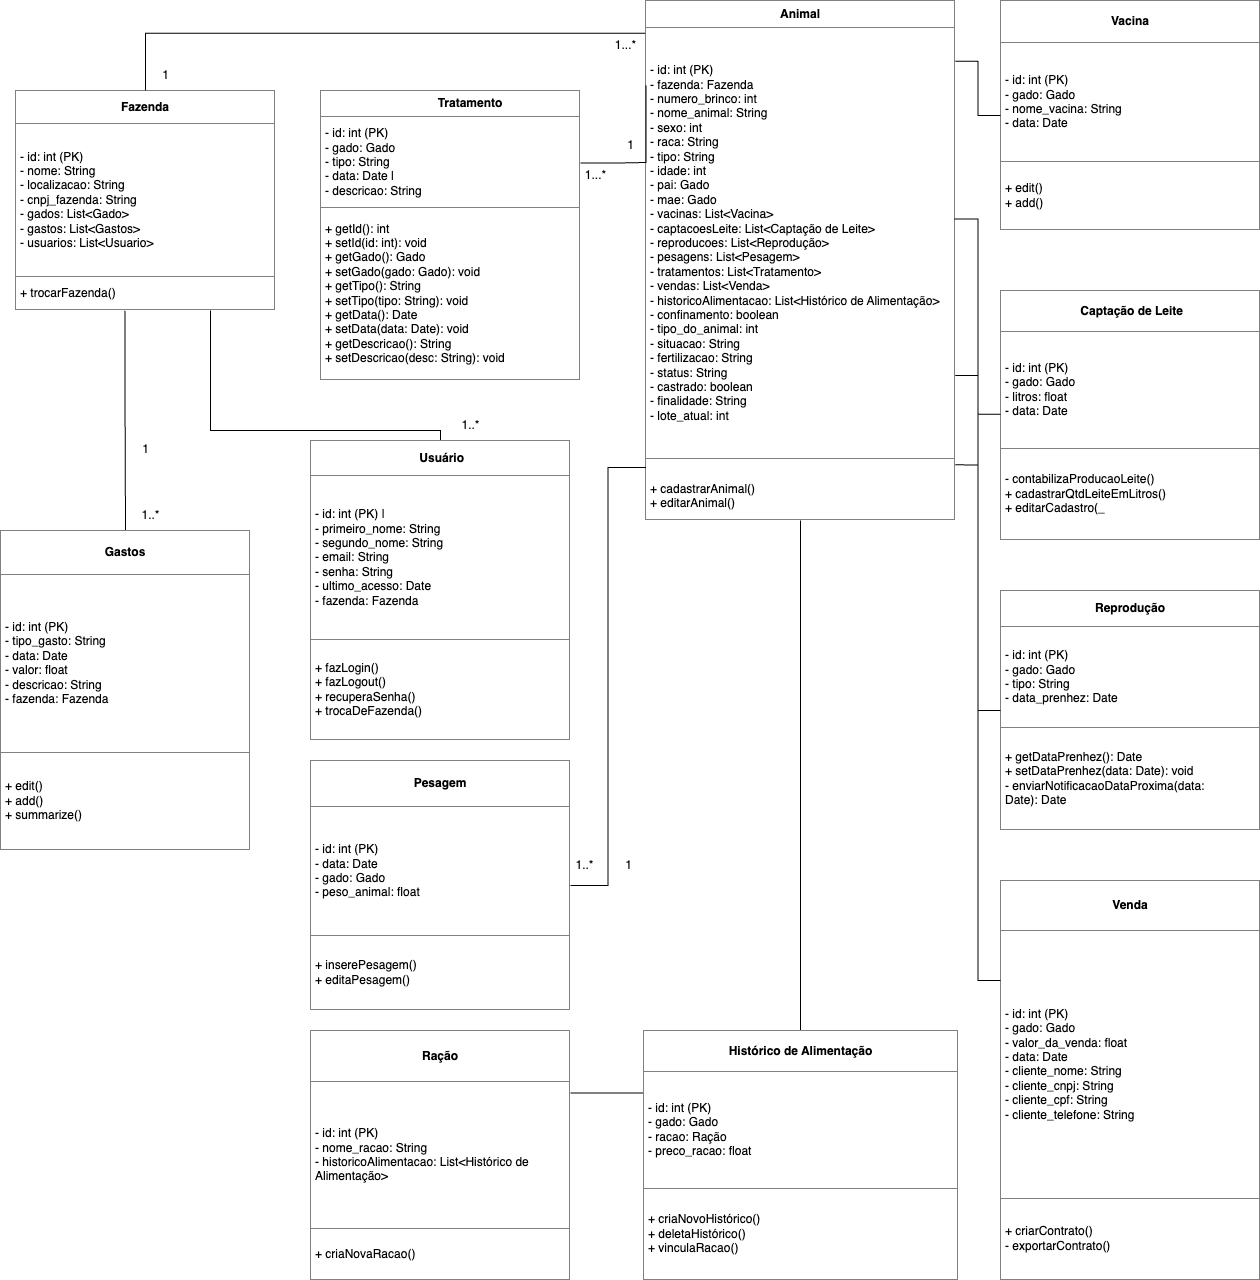
\includegraphics[width=1\textwidth]{diagrams/classesDiagram.drawio.png}
    \caption{Diagrama de Classes}
    \label{fig:classes-diagram}
\end{figure}
\end{spacing}

\subsection{Modelo Lógico}
\begin{spacing}{1.5}
O modelo lógico está apresentado na Figura \ref{fig:entity-relationship}, e reproduzido abaixo. Com o modelo lógico é criada toda a regra de negócio. Ele se refere às tabelas do banco de dados.
\begin{figure}[H]
\centering
\includegraphics[width=1\textwidth]{images/modelo-logico.drawio-1.png}
\caption{Modelo Lógico}
\label{fig:entity-relationship}
\end{figure}
\end{spacing}

\subsection{Considerações de Design}
\subsubsection{Visão Inicial da Arquitetura}
\begin{spacing}{1.5}
O projeto adota uma arquitetura modular, equilibrando a simplicidade de um monolito com a flexibilidade de serviços. O NestJS facilita a organização em módulos, permitindo escalabilidade futura para extração de serviços, como notificações. Essa escolha, juntamento com Go, suporta a gestão eficiente de rebanhos, com foco na pecuária leiteira, mantendo a robustez para expansão.
\end{spacing}

\subsubsection{Padrões de Arquitetura}
\begin{spacing}{1.5}
O projeto utiliza uma arquitetura limpa baseada em DDD (Domain-Driven Design) com arquitetura hexagonal, garantindo separação de responsabilidades e manutenção facilitada.
\end{spacing}

\begin{lstlisting}[language=bash, caption={Estrutura de Diretórios do Projeto}]
fazendapro-api/
├── api/
│   ├── handlers/
│   │   ├── user.go
│   │   └── product.go
│   └── middleware/
│       └── auth.go
├── cmd/
│   └── app/
│       └── main.go
├── config/
│   └── config.go
├── internal/
│   ├── models/
│   │   ├── user.go
│   │   └── product.go
│   ├── repository/
│   │   ├── user_repository.go
│   │   └── product_repository.go
│   └── service/
│       ├── user_service.go
│       └── product_service.go
├── pkg/
│   └── jwt/
│       └── jwt.go
├── scripts/
├── tests/
│   ├── handlers/
│   ├── repository/
│   └── service/
├── .env
├── go.mod
├── go.sum
└── README.md
\end{lstlisting}

\subsubsection{Modelo C4 — Diagrama de Contexto, Containers e Componentes}
\begin{spacing}{1.5}
Na Figura \ref{fig:C4-Contexto} é apresentado o Diagrama de Contexto, ilustrando as interações do sistema FazendaPro com atores externos, como o usuário (produtor) e serviços de notificações (WhatsApp).

\begin{figure}[H]
    \centering
    \includegraphics[width=0.2\textwidth]{images/c1.drawio.png}
    \caption{Modelo C4 — Diagrama de Contexto do sistema FazendaPro}
    \label{fig:C4-Contexto}
\end{figure}

\vspace{0.5cm}

Na Figura \ref{fig:C4-Containers} é detalhado o Diagrama de Containers, descrevendo os componentes de software, como frontend, backend, banco de dados, cache, monitoramento e pipeline de deploy, com ênfase na interação com a gestão de rebanhos e produção leiteira.

\begin{figure}[H]
    \centering
    \includegraphics[width=0.8\textwidth]{diagrams/c2.drawio.png}
    \caption{Modelo C4 — Diagrama de Containers do sistema FazendaPro}
    \label{fig:C4-Containers}
\end{figure}

\vspace{0.5cm}

Na Figura \ref{fig:C4-Componentes} é apresentado o Diagrama de Componentes, detalhando os módulos do API Server, incluindo autenticação, gerenciamento de animais, vacinas, lotes, prenhez, vendas e dashboards analíticos, com foco na rastreabilidade e produção leiteira.

\begin{figure}[H]
    \centering
    \includegraphics[width=1\textwidth]{diagrams/c3.drawio.png}
    \caption{Modelo C4 — Diagrama de Componentes do sistema FazendaPro}
    \label{fig:C4-Componentes}
\end{figure}
\end{spacing}

\subsubsection{Aplicação Web}
\begin{spacing}{1.5}
A aplicação web será desenvolvida com React, enquanto o API Server, hospedado em container no Google Cloud Run, utilizará NestJS, Go com Memcached para caching em memória, garantindo desempenho na gestão de dados pecuários.
\end{spacing}

\subsubsection{Armazenamento Persistente de Dados}
\begin{spacing}{1.5}
O armazenamento utiliza Cloud SQL (PostgreSQL). A aplicação web realiza requisições HTTP (REST) ao API Server, que consulta o Cloud SQL via conexão SQL e utiliza Memcached para caching, otimizando o acesso a dados de rebanhos e produção leiteira.
\end{spacing}


\end{spacing}

\subsection{Stack Tecnológica}
\begin{spacing}{1.5}
\subsubsection{Linguagens de Programação}
As linguagens Go, TypeScript e JavaScript foram escolhidas para serem padrões no projeto por sua eficiência, tipagem estática e adequação ao desenvolvimento web.


\subsubsection{Frameworks e Bibliotecas}
\begin{enumerate}[label=\alph*)]
\item \textbf{React} – Biblioteca JavaScript para construção de interfaces de usuário.
\item \textbf{Nest.js} – Framework backend para Node.js com foco em arquitetura escalável.
\item \textbf{TypeORM} – ORM que facilita a manipulação de bancos de dados com TypeScript.
\item \textbf{Go} – Linguagem de programação eficiente e concorrente, usada para serviços rápidos.
\item \textbf{JWT} – Padrão de token para autenticação segura entre cliente e servidor.
\item \textbf{Bcrypt} – Biblioteca para criptografia de senhas.
\item \textbf{Express} – Framework minimalista para criação de APIs com Node.js.
\item \textbf{Styled Components} – Biblioteca para estilização de componentes React com CSS-in-JS.
\item \textbf{React Router} – Gerenciador de rotas em aplicações React.
\item \textbf{React Hook Form} – Biblioteca para gerenciamento eficiente de formulários em React.
\item \textbf{React Query} – Gerencia estados de dados assíncronos (como chamadas HTTP) em React.
\item \textbf{React Toastify} – Biblioteca para exibição de notificações (toasts) em React.
\item \textbf{React Icons} – Conjunto de ícones integrável ao React.
\item \textbf{Yup} – Biblioteca de validação de esquemas, usada com formulários.
\item \textbf{Jest} – Framework de testes para JavaScript/TypeScript.
\item \textbf{Cypress} – Ferramenta de testes end-to-end para aplicações web.
\item \textbf{Tailwind CSS} – Framework utilitário para estilização com classes CSS pré-definidas.
\end{enumerate}



\subsubsection{Ferramentas de Desenvolvimento e Gestão de Projeto}
\begin{enumerate}[label=\alph*)]
\item \textbf{Podman} – Plataforma de conteinerização para empacotar e executar aplicações sem daemon.
\item \textbf{PostgreSQL} – Sistema de gerenciamento de banco de dados relacional avançado.
\item \textbf{Podman Compose} – Ferramenta para definir e executar múltiplos containers Podman.
\item \textbf{Figma} – Ferramenta colaborativa de design de interfaces e prototipação.
\item \textbf{GitHub Projects} – Ferramenta de gerenciamento de tarefas integrada ao GitHub.
\item \textbf{Google Cloud Platform} – Plataforma em nuvem para deploy escalável de aplicações.
\item \textbf{Cloud SQL} – Serviço de banco de dados PostgreSQL gerenciado na Google Cloud.
\item \textbf{Memcached} – Sistema de cache distribuído em memória de alta performance.
\item \textbf{New Relic} – Plataforma de observabilidade e monitoramento de performance de apps.
\item \textbf{Sentry} – Ferramenta para monitoramento de erros e exceções em tempo real.
\item \textbf{Mermaid} – Linguagem de marcação para criação de diagramas em texto (usada com Markdown).
\end{enumerate}

\subsubsection{Justificativa da Stack Tecnológica}
\begin{spacing}{1.5}
A escolha das tecnologias foi baseada em critérios de performance, escalabilidade e custo-benefício:

\begin{enumerate}[label=\alph*)]
\item \textbf{Go}: Escolhido para serviços de alta performance devido à baixa latência (sub-milissegundo) e eficiência em processamento concorrente, essencial para lidar com até 10.000 animais.
\item \textbf{React + TypeScript}: Garante desenvolvimento ágil com tipagem estática, reduzindo bugs em produção e facilitando manutenção.
\item \textbf{NestJS}: Arquitetura modular que facilita escalabilidade horizontal e manutenção de código.
\item \textbf{Memcached}: Cache distribuído em memória com baixa latência, otimizando consultas frequentes de dashboards. Escolhido por sua simplicidade, menor overhead de memória e excelente performance em cenários de cache distribuído.
\item \textbf{Podman}: Ferramenta de containerização sem daemon que oferece maior segurança e compatibilidade OCI, permitindo execução rootless e melhor integração com systemd.
\item \textbf{PostgreSQL}: SGBD avançado com suporte a JSON, índices GIN/GiST, transações ACID robustas e melhor conformidade com padrões SQL comparado ao MySQL.
\item \textbf{Google Cloud}: Infraestrutura escalável com auto-scaling, integração nativa com CI/CD, monitoramento avançado e SLA de 99.9%.
\end{enumerate}
\end{spacing}

\subsubsection{Análise de Custos e Alternativas}
\begin{spacing}{1.5}
\textbf{Custos Estimados (mensal):}
\begin{enumerate}[label=\alph*)]
\item \textbf{Google Cloud Run}: \$18/mês (2 vCPU, 4GB RAM, 1M requests)
\item \textbf{Cloud SQL}: \$7/mês (PostgreSQL db-f1-micro, 10GB)
\item \textbf{Memorystore}: \$13/mês (Memcached 1GB)
\item \textbf{WhatsApp Business API}: \$0.005 por mensagem (estimativa 1000 mensagens/mês = \$5)
\item \textbf{Total estimado}: \$43/mês para até 100 usuários
\end{enumerate}

\subsection{Considerações de Segurança}

\subsubsection{Conformidade com LGPD}
\begin{spacing}{1.5}
\begin{enumerate}[label=\alph*)]
    \item \textbf{Consentimento}: Implementação de mecanismo de opt-in explícito para coleta de dados sensíveis dos animais.
    \item \textbf{Direitos do titular}: Portal de autoatendimento para visualização, correção e exclusão de dados pessoais.
    \item \textbf{Minimização de dados}: Coleta apenas de dados estritamente necessários para a finalidade declarada.
    \item \textbf{Portabilidade}: Exportação de dados em formato estruturado (JSON/CSV) para facilitar migração.
\end{enumerate}
\end{spacing}

\subsubsection{Autenticação e Autorização}
\begin{spacing}{1.5}
\begin{enumerate}[label=\alph*)]
    \item \textbf{Credenciais expostas}: Senhas armazenadas com hash Bcrypt (custo 12) e salt único.
    \item \textbf{Ataques de força bruta}: Rate limiting progressivo com @nestjs/throttler (3 tentativas/min).
    \item \textbf{JWT Security}: Tokens com expiração de 15 minutos, refresh tokens com rotação.
    \item \textbf{Session Management}: Invalidação automática de sessões inativas após 30 minutos.
\end{enumerate}
\end{spacing}

\subsubsection{Criptografia e Proteção de Dados}
\begin{spacing}{1.5}
\begin{enumerate}[label=\alph*)]
    \item \textbf{Backup encryption}: Backups criptografados com chaves separadas do ambiente produtivo.
    \item \textbf{API Keys}: Armazenamento seguro de credenciais via variáveis de ambiente criptografadas.
\end{enumerate}
\end{spacing}

\subsubsection{Proteção contra Vulnerabilidades Web}
\begin{spacing}{1.5}
\begin{enumerate}[label=\alph*)]
    \item \textbf{SQL Injection}: Uso de ORM com prepared statements.
    \item \textbf{XSS}: Content Security Policy e sanitização de dados.
    \item \textbf{CSRF}: Tokens CSRF por sessão.
    \item \textbf{Input Validation}: Validação com Yup/Joi.
\end{enumerate}
\end{spacing}

\subsubsection{Logs de Auditoria e Monitoramento}
\begin{spacing}{1.5}
\begin{enumerate}[label=\alph*)]
     \item \textbf{SIEM Integration}: Integração com ferramentas de monitoramento (Sentry, New Relic).
\end{enumerate}
\end{spacing}

\subsection{Gitflow e Branches}
\begin{spacing}{1.5}
O projeto utiliza seis branches principais para ambientes de stage e produção, cobrindo serviços, backend e frontend:

\textbf{Stage:}
\begin{enumerate}[label=\alph*)]
    \item \texttt{back/develop} - backend.
    \item \texttt{front/develop} - frontend.
    \item \texttt{service/develop} - serviços.
\end{enumerate}

\textbf{Produção:}
\begin{enumerate}[label=\alph*)]
    \item \texttt{back/release} - backend.
    \item \texttt{front/release} - frontend.
    \item \texttt{service/release} - serviços.
\end{enumerate}

O fluxo de desenvolvimento envolve criar branches a partir da produção para novas funcionalidades, abrir Pull Requests para a release, testar em stage e, se aprovado, realizar o merge na produção.

% --- Próximos Passos ---
\section{Próximos Passos}
\begin{spacing}{1.5}
Os próximos passos incluem a implementação das funcionalidades descritas, com foco na construção do backend e frontend, testes de integração e validação em ambiente de stage. O cronograma será detalhado em documentos complementares, priorizando a entrega das funcionalidades principais até o final do primeiro semestre de 2025.
\end{spacing}


\begin{thebibliography}{99}

\bibitem{agro20}
CNN Brasil \textit{Agronegócio Brasileiro: entre narrativas e números}. Disponível em: \url{https://www.cnnbrasil.com.br/forum-opiniao/agronegocio-brasileiro-entre-narrativas-e-numeros/}

\bibitem{anuario2023}
EMBRAPA. \textit{Anuário Leite 2023: leite baixo carbono}. Juiz de Fora: Embrapa Gado de Leite, 2023. Disponível em: \url{https://www.embrapa.br/busca-de-publicacoes/-/publicacao/1154264/anuario-leite-2023-leite-baixo-carbono}. Acesso em: 24 jun. 2025.

\bibitem{g12022}
G1. \textit{Produtores de leite do norte de Minas enfrentam dificuldades com falta de rastreabilidade}. Disponível em: \url{https://globoplay.globo.com/v/2153861/}. Acesso em: 24 jun. 2025.

\bibitem{agropec2024}
Agrolink. \textit{Tecnologia na pecuária custa chegar ao produtor}. Disponível em: \url{https://www.agrolink.com.br/noticias/tecnologia-na-pecuaria-custa-chegar-ao-produtor_48656.html?utm_source=chatgpt.com}. Acesso em: 24 jun. 2025.

\bibitem{4milhao}
Agrolink \textit{Agronegócio Brasileiro: entre narrativas e números}. Disponível em: \url{https://www.agrolink.com.br/noticias/setor-leiteiro-emprega-cerca-de-4-milhoes-de-pessoas_465448.html}

\bibitem{lgpd2018}
BRASIL. Lei nº 13.709, de 14 de agosto de 2018. \textit{Lei Geral de Proteção de Dados Pessoais (LGPD)}. Brasília: Presidência da República, 2018. Disponível em: \url{http://www.planalto.gov.br/ccivil_03/_ato2015-2018/2018/lei/l13709.htm}. Acesso em: 24 jun. 2025.

\bibitem{anpd2024}
ANPD - Autoridade Nacional de Proteção de Dados. \textit{Guia de boas práticas para tratamento de dados pessoais}. Brasília: ANPD, 2024. Disponível em: \url{https://www.gov.br/anpd/pt-br}. Acesso em: 24 jun. 2025.

\end{thebibliography}

\appendix
\section{Apêndice} % Or 'Links Úteis', 'Recursos Online', etc.

\begin{enumerate}

    \item GO. \textit{Go Programming Language}. Disponível em: \url{https://go.dev}. Acesso em: 17 jun. 2025.
    \item TYPESCRIPT. \textit{The TypeScript Handbook}. Disponível em: \url{https://www.typescriptlang.org}. Acesso em: 17 jun. 2025.
    \item JAVASCRIPT. \textit{MDN Web Docs}. Disponível em: \url{https://developer.mozilla.org/pt-BR/docs/Web/JavaScript}. Acesso em: 17 jun. 2025.
    \item REACT. \textit{React Documentation}. Disponível em: \url{https://react.dev}. Acesso em: 17 jun. 2025.
    \item NESTJS. \textit{NestJS Documentation}. Disponível em: \url{https://nestjs.com}. Acesso em: 17 jun. 2025.
    \item TYPEORM. \textit{TypeORM Documentation}. Disponível em: \url{https://typeorm.io}. Acesso em: 17 jun. 2025.
    \item JWT. \textit{JSON Web Tokens}. Disponível em: \url{https://jwt.io}. Acesso em: 17 jun. 2025.
    \item BCRYPT. \textit{Bcrypt Documentation}. Disponível em: \url{https://www.npmjs.com/package/bcrypt}. Acesso em: 17 jun. 2025.
    \item EXPRESS. \textit{Express Documentation}. Disponível em: \url{https://expressjs.com}. Acesso em: 17 jun. 2025.
    \item STYLED COMPONENTS. \textit{Styled Components Documentation}. Disponível em: \url{https://styled-components.com}. Acesso em: 17 jun. 2025.
    \item REACT ROUTER. \textit{React Router Documentation}. Disponível em: \url{https://reactrouter.com}. Acesso em: 17 jun. 2025.
    \item REACT HOOK FORM. \textit{React Hook Form Documentation}. Disponível em: \url{https://react-hook-form.com}. Acesso em: 17 jun. 2025.
    \item REACT QUERY. \textit{React Query Documentation}. Disponível em: \url{https://tanstack.com/query}. Acesso em: 17 jun. 2025.
    \item REACT TOASTIFY. \textit{React Toastify Documentation}. Disponível em: \url{https://fkhadra.github.io/react-toastify/}. Acesso em: 17 jun. 2025.
    \item REACT ICONS. \textit{React Icons Documentation}. Disponível em: \url{https://react-icons.github.io/react-icons/}. Acesso em: 17 jun. 2025.
    \item YUP. \textit{Yup Documentation}. Disponível em: \url{https://github.com/jquense/yup}. Acesso em: 17 jun. 2025.
    \item JEST. \textit{Jest Documentation}. Disponível em: \url{https://jestjs.io}. Acesso em: 17 jun. 2025.
    \item CYPRESS. \textit{Cypress Documentation}. Disponível em: \url{https://www.cypress.io}. Acesso em: 17 jun. 2025.
    \item TAILWIND CSS. \textit{Tailwind CSS Documentation}. Disponível em: \url{https://tailwindcss.com}. Acesso em: 17 jun. 2025.
    \item PODMAN. \textit{Podman Documentation}. Disponível em: \url{https://podman.io}. Acesso em: 17 jun. 2025.
    \item POSTGRESQL. \textit{PostgreSQL Documentation}. Disponível em: \url{https://www.postgresql.org}. Acesso em: 17 jun. 2025.
    \item PODMAN COMPOSE. \textit{Podman Compose Documentation}. Disponível em: \url{https://docs.podman.io/en/latest/markdown/podman-compose.1.html}. Acesso em: 17 jun. 2025.
    \item FIGMA. \textit{Figma Documentation}. Disponível em: \url{https://www.figma.com}. Acesso em: 17 jun. 2025.
    \item GITHUB PROJECTS. \textit{FazendaPro Project}. Disponível em: \url{https://github.com/orgs/fazendapro/projects/1}. Acesso em: 17 jun. 2025.
    \item GOOGLE CLOUD. \textit{Google Cloud Documentation}. Disponível em: \url{https://cloud.google.com/docs}. Acesso em: 17 jun. 2025.
    \item CLOUD RUN. \textit{Cloud Run Documentation}. Disponível em: \url{https://cloud.google.com/run/docs}. Acesso em: 17 jun. 2025.
    \item CLOUD SQL. \textit{Cloud SQL Documentation}. Disponível em: \url{https://cloud.google.com/sql/docs}. Acesso em: 17 jun. 2025.
    \item MEMORYSTORE. \textit{Memorystore Documentation}. Disponível em: \url{https://cloud.google.com/memorystore/docs}. Acesso em: 17 jun. 2025.
    \item MEMCACHED. \textit{Memcached Documentation}. Disponível em: \url{https://memcached.org}. Acesso em: 17 jun. 2025.
    \item NEW RELIC. \textit{New Relic Documentation}. Disponível em: \url{https://newrelic.com}. Acesso em: 17 jun. 2025.
    \item SENTRY. \textit{Sentry Documentation}. Disponível em: \url{https://sentry.io}. Acesso em: 17 jun. 2025.
    \item MERMAID. \textit{Mermaid Documentation}. Disponível em: \url{https://mermaid.js.org}. Acesso em: 17 jun. 2025.
    \item C4 MODEL. \textit{C4 Model Documentation}. Disponível em: \url{https://c4model.com}. Acesso em: 17 jun. 2025.
    \item NESTJS THROTTLER. \textit{NestJS Throttler Documentation}. Disponível em: \url{https://docs.nestjs.com/techniques/throttler}. Acesso em: 17 jun. 2025.
    \item WHATSAPP WEB JS. \textit{WhatsApp Web.js Documentation}. Disponível em: \url{https://wwebjs.dev}. Acesso em: 17 jun. 2025.
\end{enumerate}

\clearpage

% --- Avaliações de Professores ---
\section{Avaliações de Professores}
\begin{spacing}{1.5}
\textbf{Considerações do Professor/a:}

\vspace{5cm}

\rule{0.5\textwidth}{0.4pt}

\vspace{1cm}

\textbf{Considerações do Professor/a:}

\vspace{5cm}

\rule{0.5\textwidth}{0.4pt}

\vspace{1cm}

\textbf{Considerações do Professor/a:}

\vspace{5cm}

\rule{0.5\textwidth}{0.4pt}
\end{spacing}

\end{document}